\documentclass{beamer}

\usetheme{CambridgeUS}

\usepackage{listings}
\usepackage{amssymb}
%\usepackage[cmex10]{amsmath}

\usepackage[export]{adjustbox}
\usepackage{bm}
\def\inputGnumericTable{} 

\usepackage[latin1]{inputenc}                                 
\usepackage{color}                                            
\usepackage{array}   
\usepackage{longtable}
\usepackage{enumitem}
\usepackage{calc}                                             
\usepackage{multirow}                                         
\usepackage{hhline}                                           
\usepackage{ifthen}  
\usepackage{mathtools}
\usepackage{tikz}
\usepackage{listings}
\usepackage{color}                                            %%
\usepackage{array}                                            %%
\usepackage{caption} 
\usepackage{graphicx}
\graphicspath{{images/}}
\captionsetup[table]{skip=3pt} 

 

\title{A1110 Assignment 10}
\author{Tejal Kulkarni \\ CS21BTECH11058 \\\vspace*{20pt} Papoullis Text Book }

\begin{document}

%\newcommand{\solution}{\noindent \textbf{Solution: }}
\providecommand{\pr}[1]{\ensuremath{\Pr\left(#1\right)}}
\providecommand{\cdf}[2]{\ensuremath{\text{F}_{#1}\left(#2\right)}}
\providecommand{\qfunc}[1]{\ensuremath{Q\left(#1\right)}}
\providecommand{\sbrak}[1]{\ensuremath{{}\left[#1\right]}}
\providecommand{\lsbrak}[1]{\ensuremath{{}\left[#1\right.}}
\providecommand{\rsbrak}[1]{\ensuremath{{}\left.#1\right]}}
\providecommand{\brak}[1]{\ensuremath{\left(#1\right)}}
\providecommand{\lbrak}[1]{\ensuremath{\left(#1\right.}}
\providecommand{\cbrak}[1]{\ensuremath{\left\{#1\right\}}}
\providecommand{\lcbrak}[1]{\ensuremath{\left\{#1\right.}}
\providecommand{\rcbrak}[1]{\ensuremath{\left.#1\right\}}}
\newcommand*{\permcomb}[4][0mu]{{{}^{#3}\mkern#1#2_{#4}}}
\newcommand*{\perm}[1][-3mu]{\permcomb[#1]{P}}
\newcommand*{\comb}[1][-1mu]{\permcomb[#1]{C}}
\renewcommand{\thetable}{\arabic{table}}


\begin{frame}
    \titlepage
\end{frame}

\begin{frame}{Outline}
  \tableofcontents
\end{frame}

\section{Question}
\begin{frame}{Question}
    \textbf{Example 6-21:}Suppose x and y are independent uniformly distributed random variables in the interval $\brak{0,\theta}$.Define $z = \text{min}(x, y)$, $w = \text{max}(x, y)$.Determine $f_{zw}\brak{z,w}$.
\end{frame}

\section{Solution}
\begin{frame}{Solution}
Both z and w vary in the interval \brak{0,\theta}.Thus,
\begin{equation}
 F_{zw}\brak{z,w} = 0    
\end{equation}
if $z < 0$ or $w < 0$
\begin{align}
   F_{zw}\brak{z,w} &= P\cbrak{z \leq z , w \leq w} \\
                    &=  P\cbrak{min(x,y) \leq z, max (x, y) \leq w} 
\end{align}
\end{frame}

\begin{frame}{}
We must consider 2 cases: $w \geq z$ and $w < z$ as shown in the figure
\begin{figure}[!ht]
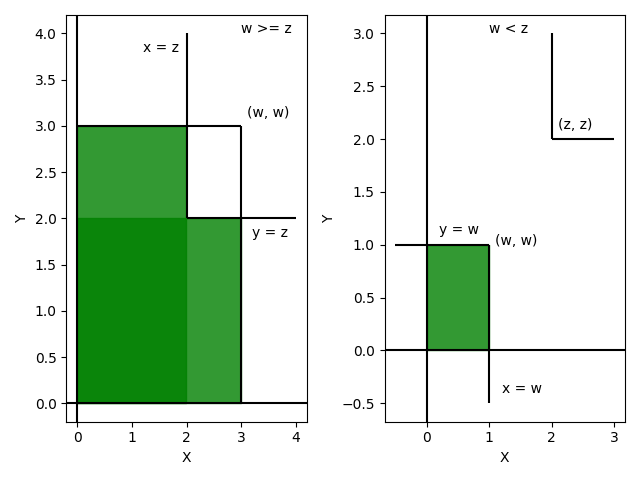
\includegraphics[scale = 0.5]{Graph.png}
\caption{a) $w\geq z$ and b) $w < z$}
\label{Fig 1}
\end{figure}
\end{frame}

\begin{frame}{}
   Case 1:$w \geq z$
\begin{equation}
    F_{zw}\brak{z,w} = F_{xy}\brak{z,w} + F_{xy}\brak{w,z} - F_{xy}\brak{z,z}
\end{equation}
Case 2: $w < z$
\begin{equation}
    F_{zw}\brak{z,w} = F_{xy}\brak{w,w}
\end{equation}
\end{frame}

\begin{frame}{}
    with
\begin{align}
   F_{xy}\brak{x,y} &= F_{x}\brak{x} F_{y}\brak{y} \\ 
                    &= \frac{x}{\theta}\times \frac{y}{\theta} \\
                    &= \frac{xy}{\theta^2}
\end{align}
we obtain,
\begin{align}
 F_{zw}\brak{z,w} = 
\begin{cases}
\brak{2wz - z^2}/\theta^2, & 0 < z < w < \theta \\
w^2/\theta^2, & 0 < w < z < \theta 
\end{cases}
\end{align}
\end{frame}

\begin{frame}{}
    Thus, 
\begin{align}  \label{eq:10}
f_{zw}\brak{z,w} = 
\begin{cases}
2/\theta^2, & 0 < z < w < \theta \\
0, & \text{otherwise}
\end{cases}
\end{align}
By equation \eqref{eq:10}, \\
Case 1: $0 < z < \theta$
\begin{align}
    f_{z}\brak{z} &= \int_{z}^{\theta} f_{zw}\brak{z,w} \,dw  \\
                  &= \frac{2}{\theta}\brak{1-\frac{z}{\theta}}  
\end{align}
Case 2: $0 < w < \theta$
\begin{align}
    f_{w}\brak{w} &= \int_{0}^{w} f_{zw}\brak{z,w} \,dz  \\
                  &= \frac{2w}{\theta^2}
\end{align}

\end{frame}

\end{document}
